\begingroup
\setlength{\tabcolsep}{0pt}
%\renewcommand{\arraystretch}{0.55} % Default value: 1
%\setlength{\fboxsep}{1mm}
\begin{table*}[t]
\centering
\begin{tabular}{|P{2cm}|P{1.3cm}|P{2cm}|L{1.3cm} P{1.7cm} D |P{8cm}|}
\hline
Technique & Interval & Reduction & Data & AvgN$_{L2}$ & Cell  & \multirow{2}{*}{Scatter Plot} \\
& & & & & Side\% & \\
\hline
\multicolumn{6}{l}{\textbf{          Cloverleaf3D Proxy Hydrodynamics Application }} & \multirow{12}{*}{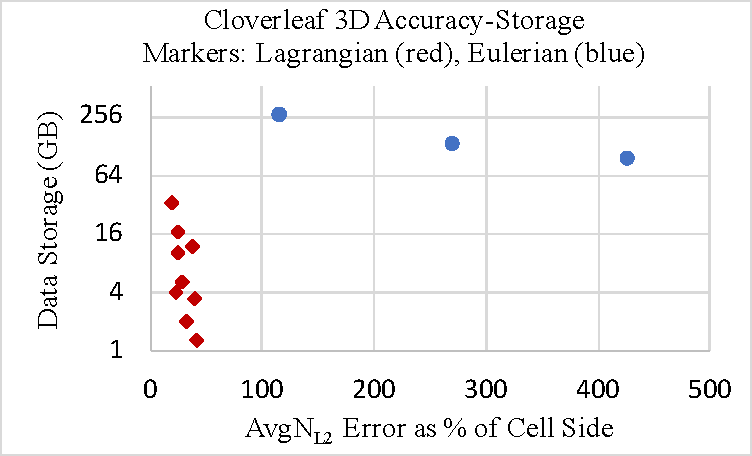
\includegraphics[width=0.95\linewidth]{images/cloverleaf_accuracy.pdf}}\\
\cline{1-6}
\multirow{3}{*}{Eulerian} & 20 & \multirow{3}{*}{Full Res} & 267 GB & 0.0197 & 116.17 &  \\
\cline{2-2}
& 40 & & 133 GB & 0.0459 & 270.49 & \\
\cline{2-2}
& 60 & & 95 GB & 0.0725 & 426.96 &  \\
\cline{1-6}
\multirow{9}{*}{Lagrangian} & \multirow{3}{*}{20} & 1:8 & 34 GB & 0.0032 & 18.928 & \\
\cline{3-3}
 & & 1:27 & 10 GB & 0.0040 & 23.891 & \\
\cline{3-3}
 & & 1:64 & 4 GB & 0.0040 & 23.583 & \\
\cline{2-3}
& \multirow{3}{*}{40} & 1:8 & 17 GB & 0.0043 & 25.646 &  \\
\cline{3-3}
& & 1:27 & 5.1 GB & 0.0049 & 29.145 &  \\
\cline{3-3}
& & 1:64 & 2 GB & 0.0053 & 31.353 & \\
\cline{2-3}
& \multirow{3}{*}{60} & 1:8 & 12 GB & 0.0064 & 37.882 & \\
\cline{3-3}
& & 1:27 & 3.4 GB & 0.0066 & 39.002 & \multirow{6}{*}{\raisebox{-33.5mm}[0pt][0pt]{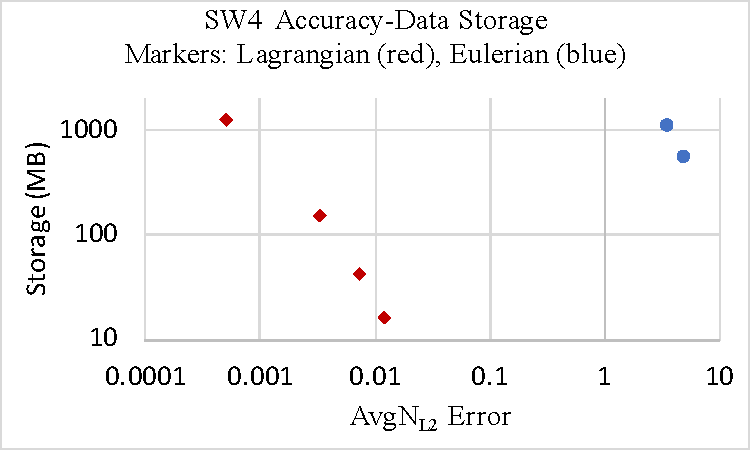
\includegraphics[width=0.95\linewidth]{images/sw4_accuracy.pdf}}} \\
\cline{3-3}
& & 1:64 & 1.3 GB & 0.0070 & 41.247 & \\
\cline{1-6}
\multicolumn{6}{l}{\textbf{          SW4 Seismic Wave Modeling Simulation }} &  \\
\cline{1-6}
\multirow{2}{*}{Eulerian} & 250 & \multirow{2}{*}{Full Res} & 1100 MB & 3.5714 & 0.9224 & \\
\cline{2-2}
 & 500 & & 550 MB & 5.0493 & 1.3023  & \\
\cline{1-6}
\multirow{4}{*}{Lagrangian} & \multirow{4}{*}{250} & 1:1 & 1300 MB & 0.0005 & 0.0001  &  \\
\cline{3-3}
 &  & 1:8 & 158 MB & 0.0033 & 0.0008 &  \\
\cline{3-3}
 &  & 1:27 & 42 MB & 0.0072 & 0.0018 & \\
\cline{3-3}
 &  & 1:64 & 16 MB & 0.0128 & 0.0031 &  \\
\cline{1-6}
\multicolumn{6}{l}{\textbf{          Nyx Cosmology Simulation }} & \\
\cline{1-6}
\multirow{4}{*}{Eulerian} & 25 & \multirow{4}{*}{Full Res} & 227 MB & 0.010 & 2.2954 &  \\
\cline{2-2}%\cline{4-6}
& 50 & & 120 MB & 0.037 & 8.4090 &  \multirow{16}{*}{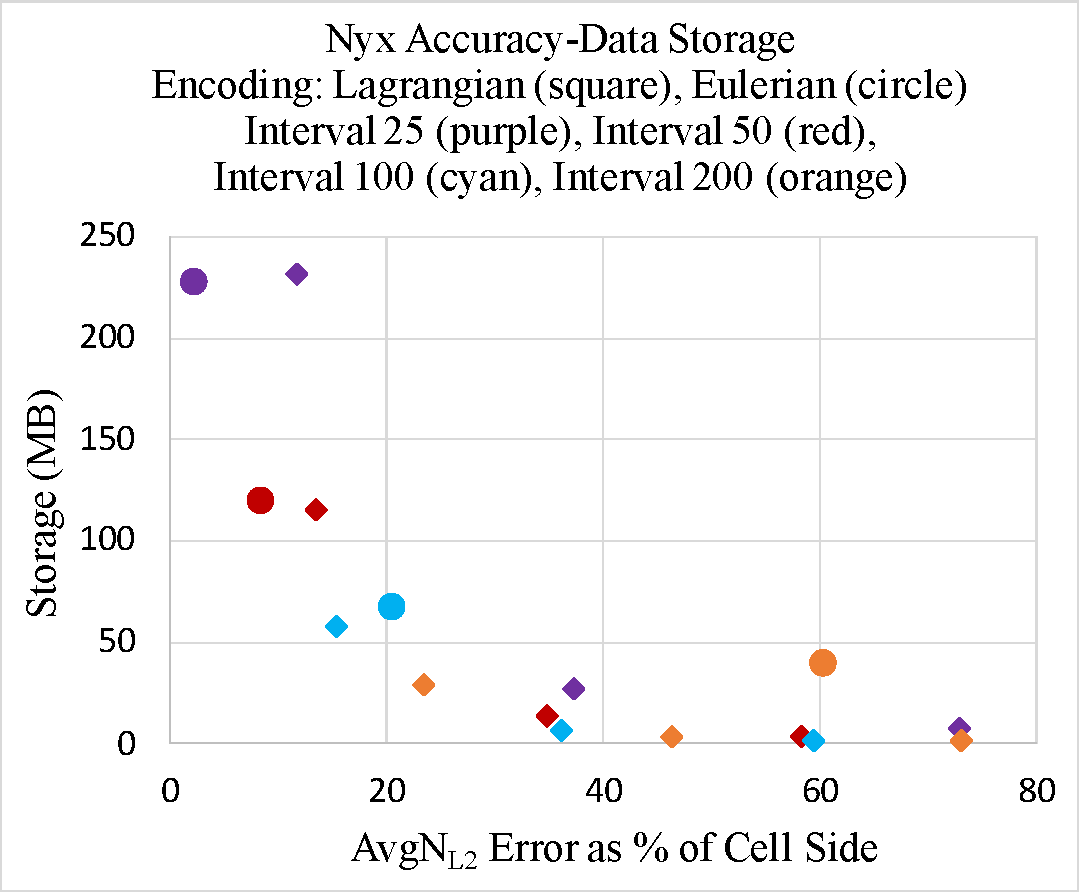
\includegraphics[width=0.95\linewidth]{images/nyx_accuracy.pdf}}\\
\cline{2-2}%\cline{4-6}
& 100 & & 67 MB & 0.090 & 20.454 & \\
\cline{2-2}%\cline{4-6}
& 200 & & 40 MB & 0.265 & 60.227 & \\
\cline{1-6}
\multirow{12}{*}{Lagrangian} & \multirow{3}{*}{25} & 1:1 & 232 MB & 0.051 & 11.613 & \\
\cline{3-3}
& & 1:8 & 27 MB & 0.164 & 37.272 &  \\
\cline{3-3}
& & 1:27 & 8 MB & 0.320 & 72.727 &  \\
\cline{2-3}
& \multirow{3}{*}{50} & 1:1 & 166 MB & 0.059 & 13.409 & \\
\cline{3-3}
& & 1:8 & 14 MB & 0.153 & 34.772 &  \\
\cline{3-3}
& & 1:27 & 4 MB & 0.256 & 58.181 &  \\
\cline{2-3}
& \multirow{3}{*}{100} & 1:1 & 58 MB & 0.067 & 15.227 &  \\
\cline{3-3}
& & 1:8 & 7 MB & 0.159 & 36.136 &  \\
\cline{3-3}
& & 1:27 & 2 MB & 0.261 & 59.318 & \\
\cline{2-3}
 & \multirow{3}{*}{200} & 1:1 & 29 MB & 0.103 & 23.409 &  \\
\cline{3-3}
& & 1:8 & 3.4 MB & 0.204 & 46.363 & \\
\cline{3-3}
& & 1:27 & 1 MB & 0.321 & 72.954 &  \\
\hline
\end{tabular}
\vspace{-3mm}
\caption{\textit{Post hoc} efficacy evaluation and experiment configurations for our three simulation codes.}
\label{table:accuracy}
\vspace{-5mm}
\end{table*}
\endgroup
